\documentclass[12pt]{article}
\usepackage[margin=2.5cm]{geometry}
\usepackage{enumerate}
\usepackage{amsfonts}
\usepackage{amsmath}
\usepackage{fancyhdr}
\usepackage{amsmath}
\usepackage{amssymb}
\usepackage{amsthm}
\usepackage{mdframed}
\usepackage{graphicx}
\usepackage{subcaption}
\usepackage{adjustbox}
\usepackage{listings}
\usepackage{xcolor}
\usepackage{booktabs}
\usepackage[utf]{kotex}
\usepackage{hyperref}
\usepackage{soul}
\usepackage{mathtools}

\definecolor{codegreen}{rgb}{0,0.6,0}
\definecolor{codegray}{rgb}{0.5,0.5,0.5}
\definecolor{codepurple}{rgb}{0.58,0,0.82}
\definecolor{backcolour}{rgb}{0.95,0.95,0.92}

\lstdefinestyle{mystyle}{
    backgroundcolor=\color{backcolour},
    commentstyle=\color{codegreen},
    keywordstyle=\color{magenta},
    numberstyle=\tiny\color{codegray},
    stringstyle=\color{codepurple},
    basicstyle=\ttfamily\footnotesize,
    breakatwhitespace=false,
    breaklines=true,
    captionpos=b,
    keepspaces=true,
    numbers=left,
    numbersep=5pt,
    showspaces=false,
    showstringspaces=false,
    showtabs=false,
    tabsize=1
}

\lstset{style=mystyle}

\pagestyle{fancy}
\renewcommand{\headrulewidth}{0.4pt}
\lhead{CSC 343}
\rhead{Assignment 1 Solution}

\begin{document}
\title{CSC343 Assignment 1 Solution}
\maketitle

\section*{Warm Up}

\begin{enumerate}[1.]
    \item What does this integrity constraint mean? $\sigma_{follower=followed}Follows = \emptyset$

    \bigskip

    \begin{mdframed}
    Means there is no result in a query where user follow himself/herself
    \end{mdframed}

    \item Would it be a good idea to define the Follows relation like this? Follows()\underline{follower}, \underline{followed}, start)

    \bigskip

    \begin{mdframed}
    Omitted for now
    \end{mdframed}

    \item Can the database represent a single post that has multiple comments?

    \bigskip

    \begin{mdframed}
        Yes.

        \bigskip

        Create two relations Comment(\underline{pid, commenter, when}, text) and
        Post(\underline{pid}, uid, when, location, caption). Set \textit{pid} in
        comment to be the \text{pid} of Post.

        \bigskip

        Since primary key of Comment is \textit{pid, commenter, when}, comments
        can have multiple entires with the same \textit{pid}.

        \bigskip

        On the other hand, since \textit{pid} in Post is the only primary key,
        it's value must be non-repeating.
    \end{mdframed}

    \item Can the database represent multiple comments from the same user on one post?

    \bigskip

    \begin{mdframed}
        Yes.

        \bigskip

        The PRIMARY KEY of Comment(\ul{pid, commenter, when}, text)
        depends on \ul{pid, commenter, when}.

        \bigskip

        By definition of PRIMARY KEY, the entry with the same pid, commenter, and when cannot exist.

        \bigskip

        Since pid and commenter are the same in this case, as long as when is different,
        the PRIMARY KEY condition will remain valid.
    \end{mdframed}

    \item How does the schema allow \textit{any} number of photos or videos to be
    inclyded in one story, but restrict the user to having only one profile photo?

    \bigskip

    \begin{mdframed}

    The user is restricted to having one profile photo since the attribute
    \textit{photo} contains only the URL of user photo.

    \bigskip

    On the other hand, a story is allowed to have multiple videos or photos, since
    its list of video and photo urls are defined in relation SIncludes, and it's PRIMARY KEY
    depends on two attributes \textit{sid} and \textit{url}.

    \bigskip

    So, as long as there are no entries in SIncludes with the repeating value of
    \textit{url}, a story can have as many photos and video urls.
    \end{mdframed}

    \item Can the database represent that a user likes the same post more than once?
    (If not, how would you change the schema to allow this?)

    \bigskip

    \begin{mdframed}

        No.

        \bigskip

        To like the same post by one person more than once, the matching values of
        the attributes \textit{liker} and \textit{pid} need to appear more than once in
        Relation Likes.

        \bigskip

        Since, \textit{pid} and \textit{liker} are together set as PRIMARY KEY, this
        is not allowed.

    \end{mdframed}

    \item Can the database represent that a user makes two posts at the same time?

    \bigskip

    \begin{mdframed}

    Yes.

    \bigskip

    For a post to be created at the same time, the date-created attribute must
    not be set as a part of primary key.

    \bigskip

    And indeed it is so in Post relation.

    \end{mdframed}

    \item  Can the database represent that the same user makes the same comment on
    two different posts?

    \bigskip

    \begin{mdframed}

    Yes.

    \bigskip

    The problem tells us the comment is made by the same user on two different posts,
    so the value of \textit{pid} is different and \textit{commenter} is the same.

    \bigskip

    Since the PRIMARY KEY of Comment relation tells us an entry cannot be created when
    \textit{pid, commenter}, and \textit{when} are the same, this doesn't create an issue.

    \bigskip

    \end{mdframed}

    \item Can the database represent that the same picture is included in 2 stories?

    \bigskip

    \begin{mdframed}

    Yes.

    \bigskip

    The problem tells us the same picture is included in two different stories,
    so the value of \textit{sid} are different and \textit{url} is the same.

    \bigskip

    Since the PRIMARY KEY of SIncludes relation tells us an entry cannot be created when
    \textit{sid}, and \textit{url} are the same, this doesn't create an issue.

    \end{mdframed}

\end{enumerate}

\section*{Part 1}

\begin{enumerate}[1.]
    \item

    \bigskip

    \underline{\textbf{Rough Work:}}

    \bigskip

    \begin{itemize}
        \item Find all users who liked a post

        \begin{mdframed}
        $\textbf{liked\_post(uid)} \coloneqq \Pi_{uid}(\rho_{\text{liker}->\text{uid}}(Likes))$
        \end{mdframed}

        \item Find all users who never liked a post

        \begin{mdframed}
        $\textbf{never\_liked(uid)} \coloneqq \Pi_{uid}(User) - \Pi_{uid}(\rho_{\text{liker}->\text{uid}}(Likes))$
        \end{mdframed}

        \item Find all users who never viewed a story

        \begin{mdframed}
        $\textbf{never\_viewed(uid)} \coloneqq \Pi_{uid}(User) - \Pi_{uid}(\rho_{\text{viewerid}->\text{uid}}(Saw))$
        \end{mdframed}

        \item Find all users who never liked or viewed a post or a story

        \begin{mdframed}
        $\textbf{never\_viewed\_or\_liked(uid)} \coloneqq \text{never\_liked\_post(uid)} \cup \text{never\_viewed\_story(uid)}$
        \end{mdframed}


        \item Find all users not followed

        \begin{mdframed}
        $\textbf{not\_followed(uid)} \coloneqq \Pi_{followers, followed, start}(\sigma_{\substack{User.uid = Follows.followed \land\\ User.uid != Follows.follower}}(Follows)) - Follows$
        \end{mdframed}

        \item Find all users who liked a post they do not follow

        \begin{mdframed}
        \end{mdframed}

        \item Find all users who never liked or viewed a post or a story they
        do not follow

        \begin{mdframed}
        \end{mdframed}
    \end{itemize}

    \bigskip

    \underline{\textbf{Notes:}}

    \bigskip

    \begin{itemize}
        \item Renaming
        \begin{itemize}
            \item \textbf{Syntax (Attribute renaming):} $\rho_{\text{oldName} \to \text{newName}}$
            \item e.g.

            \bigskip

            $\rho_{\text{Father} \to \text{Parent}}(\text{Paternity})$
        \end{itemize}
        \item Linear Notation for Algebraic Expressions
        \begin{itemize}
            \item Invents names for the temporary relations
            \item Works like variable in mathematical expression
            \item The name \textbf{Answer} is used for the result of the final step.

            \begin{center}
            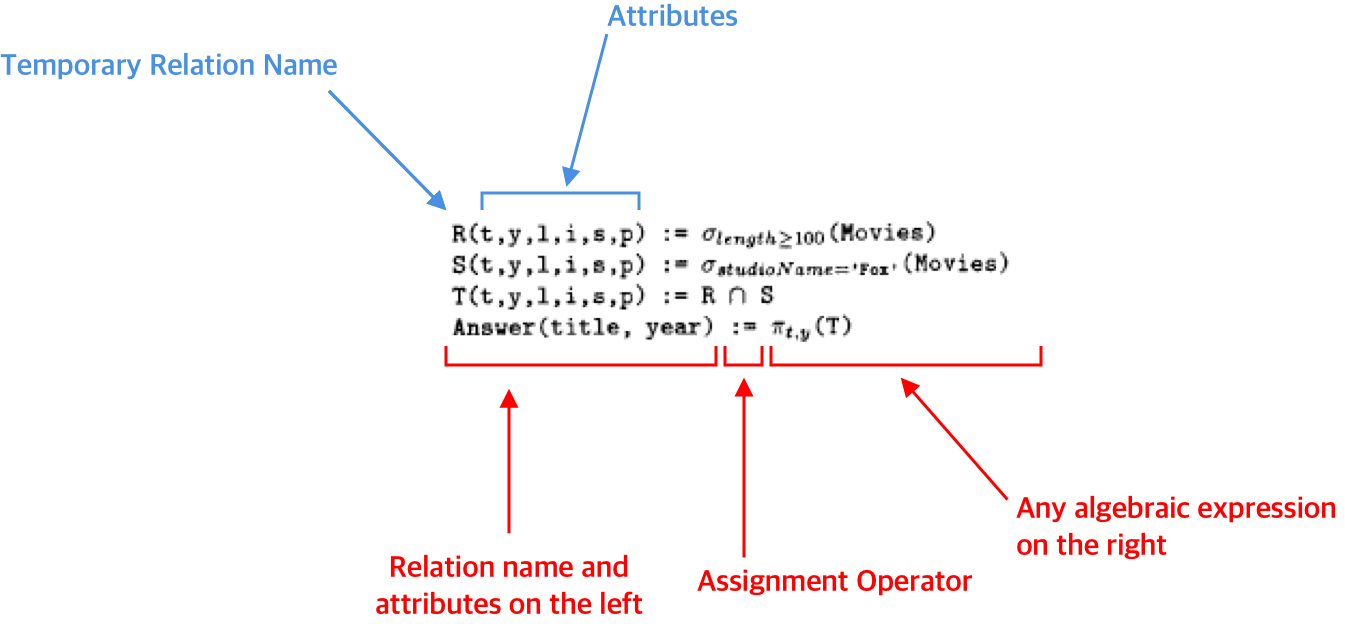
\includegraphics[width=\linewidth]{../images/assignment_1_solution_1.png}
            \end{center}
        \end{itemize}

        \item e.g. Report the user name of every student who has never worked with
        anyone, but has indeed submitted at least one file for at least one assignment

        \bigskip

        \begin{align*}
            \begin{split}
            had\_groupmates(username) &\coloneqq\\
            &\Pi_{M1.username}(\sigma_{M1.gID=M2.gID \land M1.username \neq M2.username}\\
            &(\rho_{M1}Membership \times \rho_{M2}Membership))
            \end{split}\\[1em]
            \begin{split}
            no\_groupmates(username) &\coloneqq \Pi_{username}(USER - had\_groupmates)
            \end{split}\\[1em]
            \begin{split}
            submitted\_some\_files(username) &\coloneqq \Pi_{username}(Submission)
            \end{split}\\[1em]
            \begin{split}
            \textbf{Answer(username)} &\coloneqq no\_groupmates \cap submitted\_some\_files
        \end{split}\\
        \end{align*}
    \end{itemize}

    \bigskip


\end{enumerate}

\end{document}